
\begin{answer}
\begin{figure}[H]
    \centering
    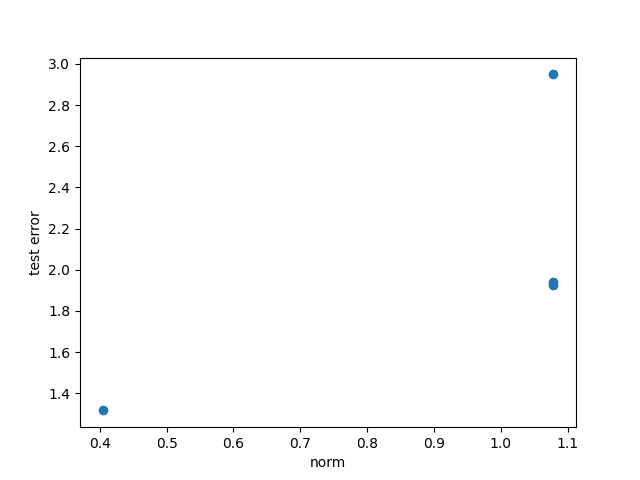
\includegraphics[width=9cm]{implicitreg/implicitreg_linear.png}
\end{figure}
From the plot, we observe that the solution with the minimum norm, $\rho$ has lower test error among the solution. That is in line with the hypothesis that the minimum norm solution should generalize well.
The other solutions were obtained by taking random vectors from the nullspace of $X$ and adding them to the min-norm solution.
\end{answer}